
\documentclass[aspectratio=169]{beamer}
\usetheme{hogent}
\usecolortheme{hgwhite} % witte achtergrond, zwarte tekst

%% common.tex -- Code die in elk .tex-bestand terug komt

%% Packages

\usepackage[dutch]{babel}
\usepackage{graphicx}
\usepackage{comment,enumerate,hyperref}
\usepackage{amsmath,amsfonts,amssymb}
\usepackage{eurosym}
\usepackage{booktabs}
\usepackage{multicol,multirow}
\usepackage{listings}

\usepackage[outputdir=out]{minted}
%\usepackage{minted}

\usepackage[backend=biber,style=apa]{biblatex}
\DeclareLanguageMapping{dutch}{dutch-apa}

\usepackage{csquotes}

%% Variabelen, elk academiejaar aan te passen
\newcommand{\academicyear}{2023--2024 (revisie: \today)}
\newcommand{\lecturers}{Thomas Aelbrecht \and Thomas Parmentier \and Bert Van Vreckem}
\newcommand{\coursename}{Research Methods (IT)}

%% Macro's en commando's

%% \alertbox: een kader voor tekst die moet opvallen
\newcommand{\alertbox}[2][hgblue]{%
  \setbeamercolor{alertbox}{bg=#1,fg=white}
  \begin{beamercolorbox}[sep=2pt,center]{alertbox}
    \textbf{#2}
  \end{beamercolorbox}
}


%---------- Info over de presentatie ------------------------------------------

\title{Module 6. Reporting research results in \LaTeX{}.}
\subtitle{\coursename}
\author{\lecturers}   % Pas waarden aan in common.tex
\date{\academicyear}

\begin{document}

\begin{frame}
  \maketitle
\end{frame}

\begin{frame}
  \frametitle{Content}

  \tableofcontents
\end{frame}

\section{Verifying installation}

\begin{frame}
  \frametitle{Does everyone have a working {\LaTeX}-installation?}

  \begin{itemize}
   \item Does paper compile to PDF?
   \item Is bibliography visible? (F5-F8-F5)
   \item Correct references in the text?
   \item Errors during compilation?
   \item Errors in the PDF file?
  \end{itemize}
  
  \bigskip
  
  \alertbox{Use the guide! \url{https://hogenttin.github.io/latex-hogent-gids/}}

\end{frame}

\section{Tips \& tricks}


\begin{frame}
  \frametitle{Verifying installation, compiler}

  \begin{itemize}
    \item Mik{\TeX} Console: check for updates
          \begin{itemize}
            \item As Administrator
            \item As regular user
          \end{itemize}
    \item Settings TeXstudio
          \begin{itemize}
            \item Compiler (\texttt{xelatex})
            \item Bibliography (\texttt{biber}/\texttt{biblatex})
          \end{itemize}
  \end{itemize}

\end{frame}

\begin{frame}
  \frametitle{Checking bibliography}

  \begin{itemize}
        \item Is the bibliography available?
       \begin{itemize}
           \item F5 - F8 - F5
           \item of: Tools > Build - Bibliography - Build
       \end{itemize}
        \item Do you see references like this in the text? (\textbf{Doe2021})
       \begin{itemize}
           \item i.e. ~Bib{\TeX}-key in bold
           \item Make sure bibliography is compiled
           \item Check Bib{\TeX}-key (output from biber)
           \item After recompiling you will see (Doe, 2021)
       \end{itemize}
  \end{itemize}

\end{frame}

\begin{frame}[fragile]
  \frametitle{Correct use of quotes}

  \textcolor{red}{\textbf{WRONG:}} \verb|"Some text"| $\Rightarrow$ \"Some text"

  \bigskip

  \textcolor{green}{\textbf{RIGHT:}} \verb|``Some text''| $\Rightarrow$ ``Some text''

  \bigskip

  Use two ``backquotes'' (left) or two single quotes (right)
\end{frame}

\begin{frame}[fragile]
    \frametitle{Be careful with special characters}
    
    \begin{itemize}
        \item Certain characters have a special meaning in {\LaTeX}
        \item Some are even prohibited in JabRef!
        \item Use commands to render these:
    \end{itemize}
    
    \bigskip
    
    \begin{center}
        \begin{tabular}{rccccc}
            \toprule
            \textbf{Symbol}  & \&        & \$        & \_        & \%  & \textbackslash{} \\
            \textbf{Command} & \verb+\&+ & \verb+\$+ & \verb+\_+ & \verb+\%+ & \verb+\textbackslash+\\
            \bottomrule
        \end{tabular}
    \end{center}
    \end{frame}
    

\begin{frame}
  \frametitle{What command for this symbol?}

  \url{https://detexify.kirelabs.org/classify.html}

  \centering
  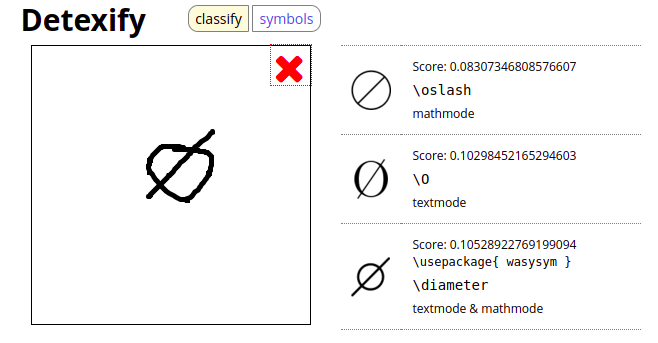
\includegraphics[height=.6\textheight]{6/detexify}

\end{frame}

\begin{frame}[fragile]
  \frametitle{Entering URLs }

  \begin{itemize}
    \item Via package \texttt{hyperref} (already loaded in template!)
    \item Commands \verb+\url{}+, \verb+\href{}{}+
    \item Hyperref also makes:
          \begin{itemize}
            \item Table of contents in the PDF
            \item Clickable references in the document
          \end{itemize}
  \end{itemize}

\end{frame}

\begin{frame}[fragile]
  \frametitle{Entering URLs: example}

  \verb+\url{https://xkcd.com/1301/}+ $\Rightarrow$ \url{https://xkcd.com/1301/}

  \bigskip

  \verb+\href{https://xkcd.com/1301/}{File Extensions}+

  $\Downarrow$

  \href{https://xkcd.com/1301/}{File Extensions}

\end{frame}

\begin{frame}[fragile]
  \frametitle{References in a document}

  \begin{itemize}
    \item You can refer to anything that has a number
    \begin{itemize}
        \item Chapter/section, figure, table, math.~equation, \ldots
    \end{itemize}
    \item Define label with \verb+\label{LABEL}+
    \item Refer to it with \verb+\ref{LABEL}+
    \item Rule of thumb: name of label reflects type, e.g. \texttt{fig:chart}, \texttt{ch:introduction}, \texttt{tab:summary}, \texttt{eq:variance}, \ldots   
  \end{itemize}

\end{frame}

\begin{frame}
  \frametitle{Overfull/underfull hbox}

  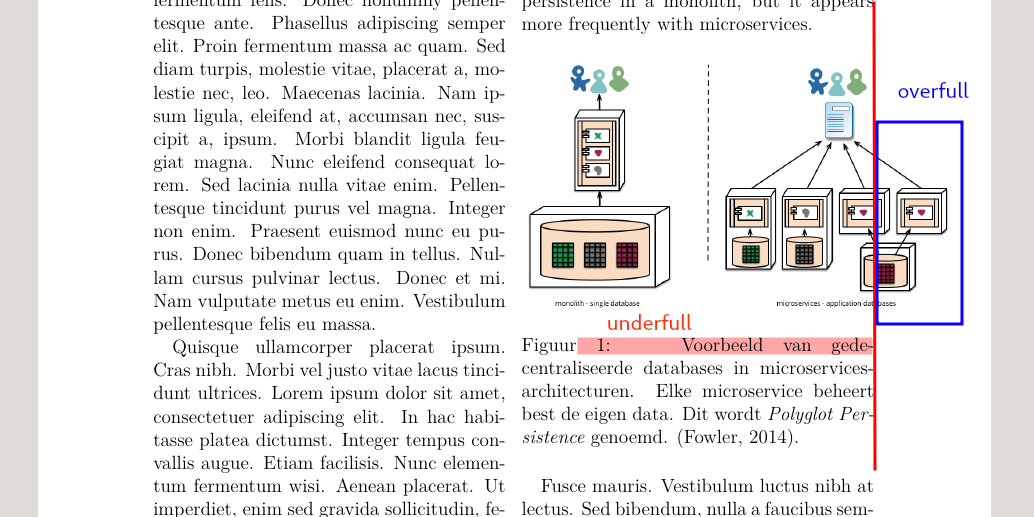
\includegraphics[height=.7\textheight]{6/hbox-warnings}

\end{frame}

\begin{frame}[fragile]
  \frametitle{Overfull/underfull hbox}
  \framesubtitle{Probably the most common compiler warning!}

  \begin{itemize}
    \item \textbf{Cause:} figure does not fit within the page margins
    \item \textbf{Solution:} rescale figure, e.g.:
  \end{itemize}

\begin{verbatim}
\includegraphics[width=.49\textwidth]{img/polygl-persist}
\end{verbatim}

\end{frame}

\begin{frame}[fragile]
  \frametitle{Overfull/underfull hbox}
   \framesubtitle{Probably the most common compiler warning!}

  \begin{itemize}
   \item \textbf{Cause:}
   \begin{itemize}
       \item Too much or too little text to fill margins nicely
       \item Usually because of a compound word, e.g. ``microservices\textcolor{red}{\textbf{--}}architectures''
       ({\LaTeX} will only split at that place)
   \end{itemize}
   \item \textbf{Solution:} Specify correct split, e.g.:
   \begin{itemize}
       \item In the text: \verb|ar\-chi\-tec\-tu\-res|
       \item Preamble: \verb|\hyphenation{ar-chi-tec-tu-res}|
    \end{itemize}
  \end{itemize}

\end{frame}

\begin{frame}[fragile]
  \frametitle{Overfull/underfull hbox}
  \framesubtitle{Probably the most common compiler warning!}

  \begin{itemize}
    \item \textbf{Cause:} URL is too long, no word split
    \item \textbf{Solution:} The \texttt{breaklinks}-option of the \texttt{hyperref}-package \footnote{This option is already included in the rm-paper template}:
  \end{itemize}

\begin{verbatim}
\usepackage[bookmarks=true,breaklinks]{hyperref}
\end{verbatim}
\end{frame}

\begin{frame}
  \frametitle{Overfull/underfull hbox}

    \textbf{Please note} It's a \emph{warning}, not a \emph{error}! Not every hbox warning needs to be fixed!

  \centering
  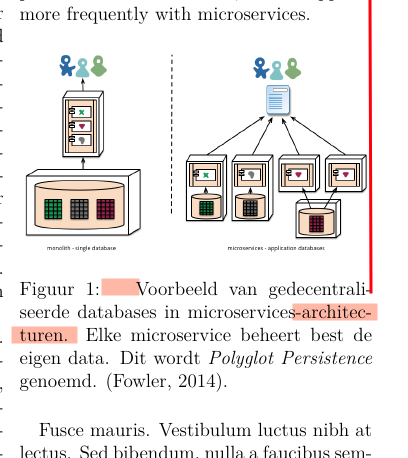
\includegraphics[height=.6\textheight]{6/hbox-fixed}

\end{frame}

\section{Floating environments}

\begin{frame}
  \frametitle{{\LaTeX} floating environments}

  \begin{itemize}
   \item = Content that belongs together should not be split
   \item E.g. image, table
   \item {\LaTeX} chooses where to place them for optimal page layout
   \item Sometimes on another page!
  \end{itemize}

\end{frame}

\begin{frame}
  \frametitle{Use of images: mistakes}

  \centering
  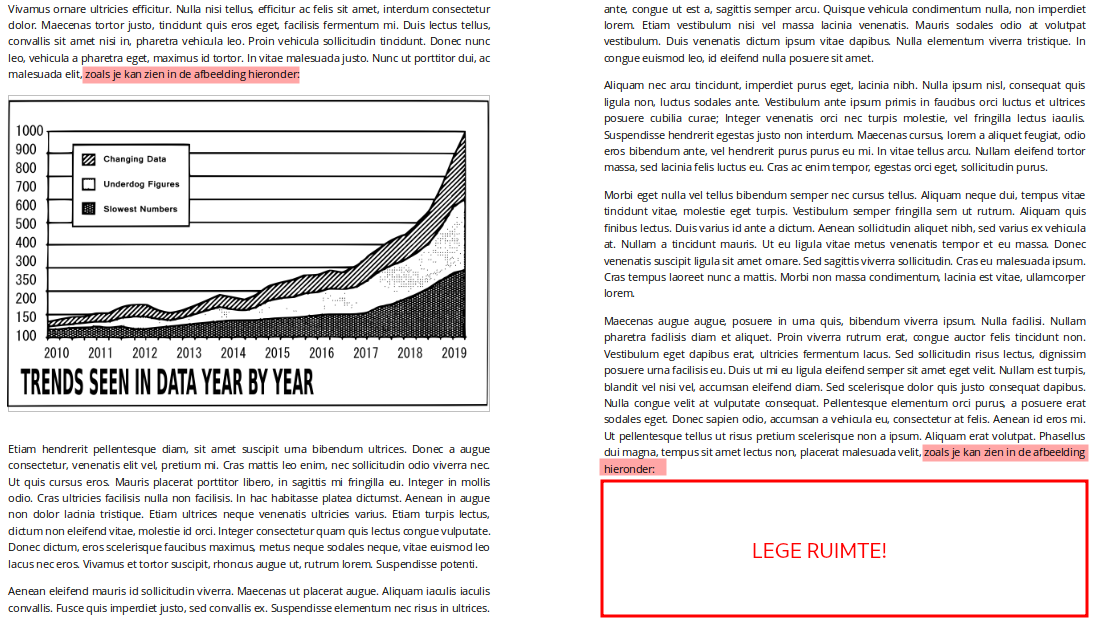
\includegraphics[height=.7\textheight]{6/afbeeldingen-tekstverwerker}

\end{frame}

\begin{frame}
  \frametitle{Images in {\LaTeX}}

  \begin{itemize}
    \item Use Figure-environment
    \item Label each image
    \item Refer to the image in the text
    \item Provide extended caption
    \item Citation if necessary!
  \end{itemize}

\end{frame}

\begin{frame}[fragile,plain]
  \frametitle{Images in {\LaTeX}}

  \begin{columns}[c]
    \column{.65\textwidth}

\begin{semiverbatim}
\small
\alert<1>{\\begin\{figure\}}
  \alert<2>{\\centering}
  \alert<3>{\\includegraphics[width=.8\\textwidth]
    \{images/chart\}}
 \alert<4>{\\caption\{\alert<5>{\\label\{fig:chart\}}We see an increasing trend in
     the data every year \alert<6>{\\autocite\{Doe2021\}}.\}}
\alert<1>{\\end\{figure\}}
\end{semiverbatim}

    \column{.35\textwidth}
    \begin{figure}
      \centering
      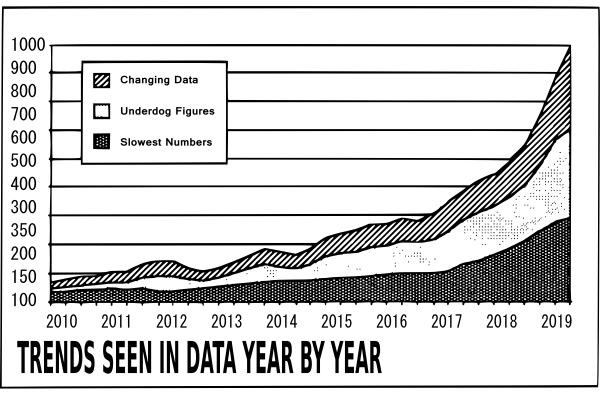
\includegraphics[width=.8\textwidth]{6/chart}
      \caption{\label{fig:chart} We see an increasing trend in the data every year (Doe, 2021).}
    \end{figure}

  \end{columns}

\end{frame}

\begin{frame}[fragile]
  \frametitle{References in the text}

  \begin{verbatim}
According to~\textcite{Doe2021} there is an increasing trend in the data every year (see Figuur~\ref{fig:chart}).
\end{verbatim}

  \[\Downarrow\]

  \bigskip

  According to Doe (2021) there is an increasing trend in 
  the data every year (see Figure 1.3).

\end{frame}

\begin{frame}
  \frametitle{Tables in {\LaTeX}}
  \framesubtitle{Example}

  \begin{table}
    \begin{tabular}{lcr}
      \toprule
      \textbf{Column 1} & \textbf{Column 2} & \textbf{Column 3} \\
      $\alpha$          & $\beta$           & $\gamma$          \\
      \midrule
      A                 & 10.230            & a                 \\
      B                 & 45.678            & b                 \\
      C                 & 99.987            & c                 \\
      \bottomrule
    \end{tabular}
    \caption{\label{tab:example}Minimal booktabs example.}
  \end{table}

\end{frame}

\begin{frame}[fragile]
  \frametitle{Tables in {\LaTeX}}
  \framesubtitle{Source code}

  \small
\begin{semiverbatim}
\alert<1>{\\begin\{table\}}
  \alert<2>{\\begin\{tabular\}}\{\alert<3>{lcr}\}
    \alert<4>{\\toprule}
    \\textbf\{Column 1\} \alert<5>{&} \\textbf\{Column 2\} \alert<5>{&} \\textbf\{Column 3\} \alert<5>{\\\\}
    \$\\alpha\$          \alert<5>{&} \$\\beta\$           \alert<5>{&} \$\\gamma\$          \alert<5>{\\\\}
    \alert<4>{\\midrule}
    A                 \alert<5>{&} 10.230            \alert<5>{&} a                 \alert<5>{\\\\}
    B                 \alert<5>{&} 45.678            \alert<5>{&} b                 \alert<5>{\\\\}
    C                 \alert<5>{&} 99.987            \alert<5>{&} c                 \alert<5>{\\\\}
    \alert<4>{\\bottomrule}
  \alert<2>{\\end\{tabular\}}
  \alert<6>{\\caption\{\\label\{tab:example\}Minimal booktabs example.\}}
\alert<1>{\\end\{table\}}
\end{semiverbatim}

\end{frame}

\begin{frame}
  \frametitle{Tips \& Tricks}

  \begin{itemize}
   \item Use \texttt{booktabs}-package for nicer tables
   \item Use \url{https://www.tablesgenerator.com}
   \item Do not use vertical lines
   \item Wide table? Rotate with \texttt{rotating} package and \texttt{sidewaystable} environment
   \item Placemarks (eg ~\texttt{[ht!]}) are usually not needed!
  \end{itemize}

\end{frame}

\begin{frame}[fragile]
  \frametitle{List of Figures/Tables}

  \begin{itemize}
    \item You can insert a list of figures and tables:
\begin{verbatim}
\listoffigures    % Figuren
\listoftables     % Tabellen
\listoflistings   % Broncode
\end{verbatim}
    \item Full caption is copied!
    \item Provide a short description:
    
      \verb|\caption[Short description]{Long caption}|
  \end{itemize}

\end{frame}

\section{Mathematical formulas}

\begin{frame}[fragile]
  \frametitle{Mathematical formulas in {\LaTeX}}

  \begin{itemize}
   \item In a sentence: \verb+$ ... $+ or \verb+\( ... \)+
   \item On one line: \texttt{equation}-environment
   \item or \verb+\[ ... \]+
  \end{itemize}

  More info in ~\href{https://tobi.oetiker.ch/lshort/lshort.pdf}{lshort} or \href{https://en.wikibooks.org/wiki/LaTeX/Mathematics}{LaTeX Wikibook}

\end{frame}

\begin{frame}[fragile]
  \frametitle{Examples}

\begin{verbatim}
  \[\overline{x} = \sum_{i=1}^{n} x_i\]
\end{verbatim}

  \bigskip

  \centering
  $\Downarrow$

  \bigskip

  \[\overline{x} = \sum_{i=1}^{n} x_i\]

\end{frame}

\begin{frame}[fragile]
  \frametitle{Examples}

\begin{verbatim}
\[s = \sqrt{\frac{1}{n-1} 
  \sum_{i=1}^{n} (x_i - \overline{x})^2} \]
\end{verbatim}

  \bigskip

  \centering
  $\Downarrow$

  \bigskip

  \[s = \sqrt{\frac{1}{n-1} \sum_{i=1}^{n} (x_i - \overline{x})^2} \]

\end{frame}

\begin{frame}
  \frametitle{Use outside {\LaTeX}}

{\LaTeX} syntax for math formulas is also used outside of {\LaTeX}!

  \begin{itemize}
   \item Python/Jupyter Notebooks
   
   eg \url{https://github.com/HoGentTIN/dsai-labs/blob/main/7-time-series/7.01-time-series.ipynb}
   
   \item In web pages: via \href{https://www.mathjax.org}{MathJax}
   
   \url{http://docs.mathjax.org/en/latest/input/tex/index.html}
   
   \item In e.g. ~reveal.js presentations
    \item \ldots
  \end{itemize}

\end{frame}

\section{Source code}

\begin{frame}[fragile]
 \frametitle{Insert source code}
 \framesubtitle{Simplest form: \texttt{verbatim}}

\begin{semiverbatim}
\alert{\\begin\{verbatim\}}
public class MyApp \{
 public static void main(String args[]) \{
   System.out.println("Hello World");
 \}
\}
\alert{\\end\{verbatim\}}
\end{semiverbatim}

  \centering
  $\Downarrow$

\begin{verbatim}
public class MyApp {
 public static void main(String args[]) {
   System.out.println("Hello World");
 }
}
\end{verbatim}

\end{frame}

\begin{frame}[fragile]
 \frametitle{Insert source code}
 \framesubtitle{\texttt{listings} package}

\begin{semiverbatim}
\\lstset\{\%
language=java,  breaklines=true,  numbers=left,
frame=single, caption=\{My first Java-program.\},
label=code:helloworld\}

\alert{\\begin\{lstlisting\}}
public class MyApp \{
 public static void main(String args[]) \{
   System.out.println("Hello World");
 \}
\}
\alert{\\end\{lstlisting\}}
\end{semiverbatim}

\end{frame}

\begin{frame}[fragile]
 \frametitle{Insert source code}
 \framesubtitle{\texttt{listings} package}

  \lstset{%
    language=java,    breaklines=true,
    numbers=left,     frame=single,
    caption={My first Java-program.},
    label=code:helloworld,
    gobble=2
  }

  \begin{lstlisting}
  public class MyApp {
    public static void main(String args[]) {
      System.out.println("Hello World");
    }
  }
  \end{lstlisting}

\end{frame}

\begin{frame}[fragile]
 \frametitle{Insert source code}
  \framesubtitle{\texttt{minted} package}

  \begin{semiverbatim}
  \\setminted\{%
    bgcolor=gray!20,gobble=2, linenos,
    numbers=left,frame=single\}

  \\begin\{minted\}\{java\}
    public class MyApp \{
      public static void main(String args[]) \{
        System.out.println("Hello World");
      \}
    \}
  \\end\{minted\}
  \end{semiverbatim}
\end{frame}

\begin{frame}[fragile]
 \frametitle{Insert source code}
  \framesubtitle{\texttt{minted} package}
  \setminted{bgcolor=gray!20,gobble=4,linenos,numbers=left,frame=single}
  \begin{minted}{java}
    public class MyApp {
      public static void main(String args[]) {
        System.out.println("Hello World");
      }
    }
  \end{minted}
  
  \bigskip
  
  Refer to \url{https://hogenttin.github.io/latex-hogent-gids/installatie-minted/}
  
\end{frame}

\section{Finally\ldots}

\begin{frame}
  \frametitle{Some recommendations}

  \begin{itemize}
   \item Do not prepare your text in Word to convert to {\LaTeX} at the end
   \item Start with minimal document that compiles
   \item Work step by step, don't add too much text/code at once!
   \item Read a manual/book!
   \item \textbf{Read the error messages carefully}
  \end{itemize}

\end{frame}

\begin{frame}
  \frametitle{Text for the future!}

 Consider moving to a text-based workflow as much as possible!

  \begin{columns}
    \begin{column}{.7\textwidth}
      \begin{itemize}
       \item Everything in Git!
       \item Notes in Markdown
       \item Data in CSV, processed with Python
       \item Reporting in LaTeX
      \end{itemize}
    \end{column}

    \begin{column}{.3\textwidth}
      
\includegraphics[height=3cm]{6/word-trashbin}
    \end{column}
  \end{columns}

  
\end{frame}

\begin{frame}
  \frametitle{Why?}

  \begin{itemize}
    \item Easier search in directory tree
    \begin{itemize}
        \item e.g.~\href{https://github.com/ggreer/the_silver_searcher}{The Silver Searcher/\texttt{ag}}
    \end{itemize}
    \item Convert to any format
    \begin{itemize}
        \item Website, presentation, PDF, \ldots
        \item \url{https://pandoc.org}
        \item \url{https://www.mkdocs.org}
        \item \url{https://pages.github.com}
    \end{itemize}
    \item Automate Workflow
    \begin{itemize}
        \item Python/Bash script can handle text!
    \end{itemize}
    \ item Future proof!
  \end{itemize}

\end{frame}

\section{Exercise, assignment}

\begin{frame}
  \frametitle{Exercise, assignment}

  \begin{itemize}
   \item Try these things out! Ask for help where needed.
   \begin{itemize}
       \item Test document or copy paper
   \end{itemize}
   \item Finish paper, see:
    
    \url{https://github.com/HoGentTIN/rm-paper-en/tree/main/instructions/6-final.md}
  \end{itemize}
\end{frame}

\end{document}
